\subsection{Uncertainties in gas chemistry}
\label{sec:uncergaschem}
Accurate simulation of soot and carbon black formation remains a major challenge due to the compounded uncertainties introduced when coupling gas-phase chemistry with soot models. Prior studies have shown that the predicted concentrations of large PAHs can vary by orders of magnitude depending on the chosen reaction mechanism~\citep{wang2023systematic}. Moreover, there are not well-established pathways and rate constants for elementary reactions governing PAH dimerization, radical interactions, and surface reactions~\citep{martin2022soot}. Consequently, soot models inherit uncertainty from two sources: (i) the reaction mechanism used to describe fuel pyrolysis and oxidation, and (ii) the choice of inception and surface growth models and parameters. The cumulative effect significantly complicates efforts to produce reliable predictions of soot mass and morphology. This highlights the importance of coupling between gas-phase chemistry and soot formation models because the reliability of soot and carbon black simulations hinges more on the accuracy of upstream chemical kinetics, inception and surface growth fluxes.

To illustrate the impact of chemical mechanism selection on precursor formation, a series of simulations\footnote{\href{https://github.com/mohammadadib-cu/omnisoot-cv/tree/main/examples/pressure/mechanism_comparison}{https://github.com/mohammadadib-cu/omnisoot-cv/tree/main/examples/pressure/mechanism\_comparison}} were performed using the CPR model of omnisoot (with soot formation disabled) for the pyrolysis of $5\%$ $\mathrm{CH_4}$-Ar mixture at $\mathrm{T_5}=$2203 K and $\mathrm{P_5}=$4.9 atm~\hl{[GB]}. Six widely used chemical mechanisms were evaluated: ABF~\citep{appel2000kinetic}, Caltech~\citep{blanquart2009chemical}, KAUST~\citep{wang2013pah}, CRECK~\citep{saggese2015kinetic}, ITV~\citep{hellmuth2024role}, and FFCM2~\citep{ZDV2023}.

The comparison focuses on the mole fraction of small intermediates, and soot volume fraction measured using continuous wave absorption and laser extinction at 632 nm, respectively~\hl{[GB]}. Figure~\ref{fig:CH4_C2H2_C2H4_chem} shows the large variability in the predicted mole fraction of $\mathrm{CH_4}$, $\mathrm{C_2H_2}$, and $\mathrm{C_2H_4}$ across different reaction mechanisms. The mole fraction of $\mathrm{CH_4}$ serves as a useful indicator of carbon flux from the fuel to small and large intermediates. Our carbon flux analysis, performed for all the mechanisms, highlighted the major role of $\mathrm{C_2H_4}$ in the production of $\mathrm{C_2H_2}$ via vinyl radical ($\mathrm{C_2H_3}$) as shown in prior studies (Figure~10 in \citep{wang2023systematic}). 

As shown in the inset of Figure~\ref{fig:CH4_C2H2_C2H4_chem}a, the CRECK mechanism predicts the lowest $\mathrm{CH_4}$ mole fraction (i.e., the largest conversion) at residence times up to 0.5 ms, whereas the KAUST mechanism yields a lower mole fraction conversion at longer residence times. Both mechanisms significantly underpredict methane mole fraction compared to the measurements. ABF and FFCM2 provide more accurate prediction of the $\mathrm{CH_4}$ considering the uncertainty of the experimental data. As shown in the inset of Figure~\ref{fig:CH4_C2H2_C2H4_chem}b, CRECK and KAUST mechanisms overpredict the initial jump in the mole fraction of  $\mathrm{C_2H_4}$. A similar variability can be observed in the prediction of $\mathrm{C_2H_2}$ mole fraction: it is best captured by FFCM2, overpredicted by CRECK, and underpredicted by the other kinetic mechanisms. FFCM2 (denoted by solid dashed line in Figure~\ref{fig:CH4_C2H2_C2H4_chem}) is overall in better agreement with measurements, but this mechanism only considers $\mathrm{C_1}-\mathrm{C_4}$ species not benzene and larger PAHs, so it cannot be coupled with the soot models considered in this study.
 
\begin{figure}[H]
	\centering
	\begin{subfigure}[t]{0.32\textwidth}
		\begin{tikzpicture}
			\draw (0, 0) node[inner sep=0] 	{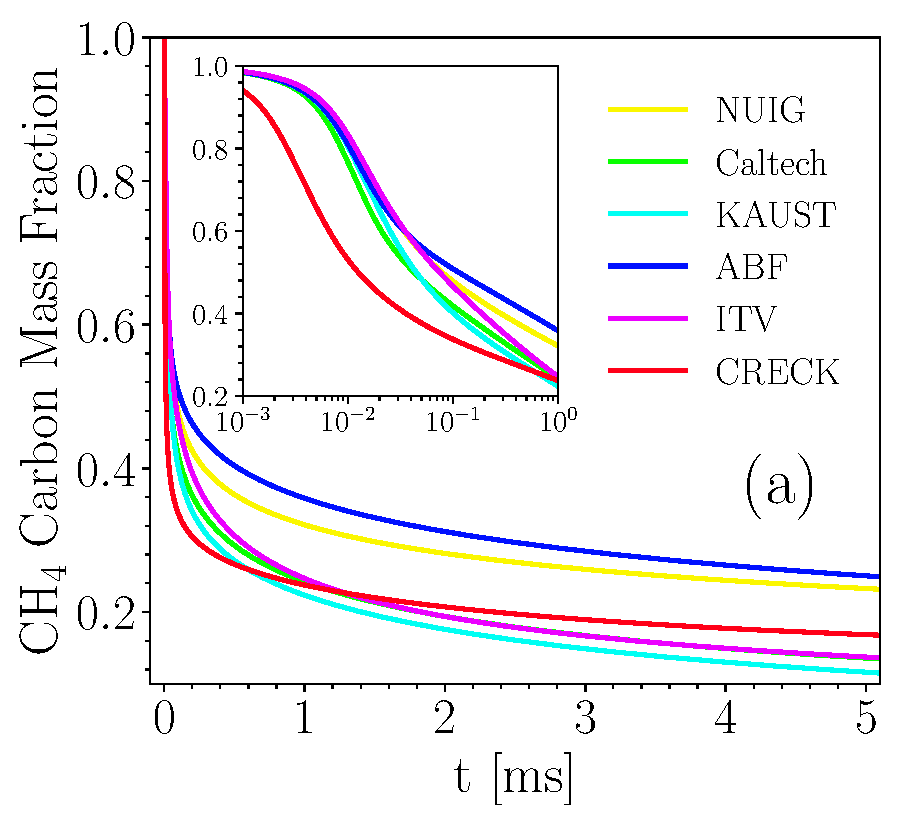
\includegraphics[width=1\textwidth]{Figures/Results/chemistry/CH4.pdf}};
			\draw (1.75, 1.82) node {\tiny{\hl{[G]}}};
		\end{tikzpicture}
	\end{subfigure}
	\begin{subfigure}[t]{0.32\textwidth}
		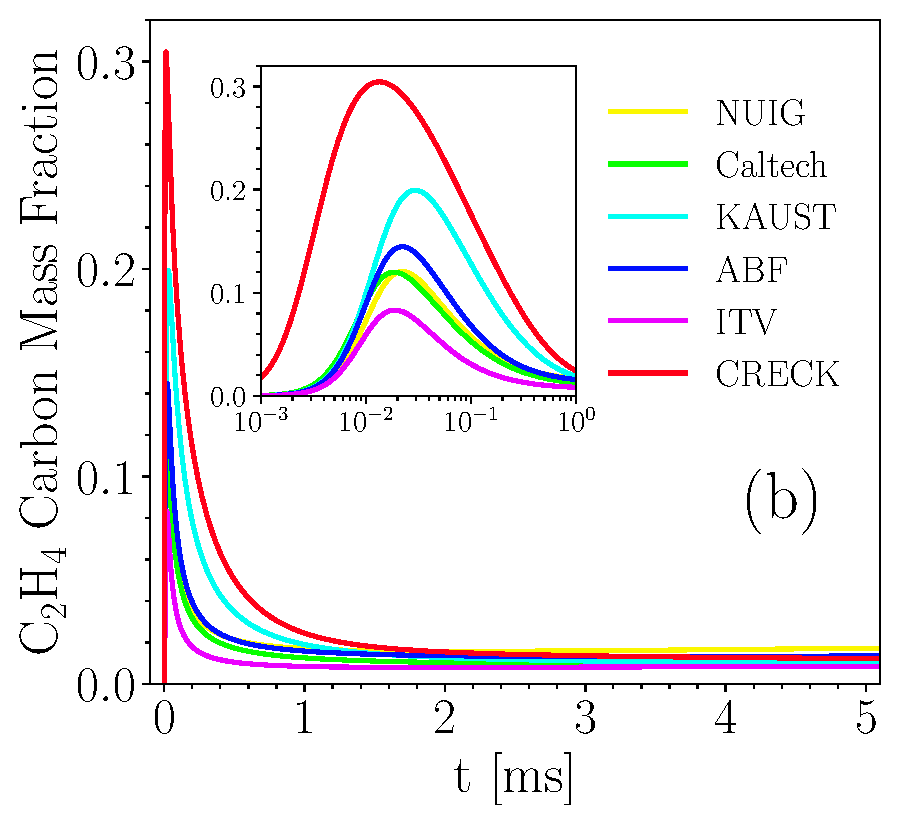
\includegraphics[width=1\textwidth]{Figures/Results/chemistry/C2H4.pdf}
	\end{subfigure}
	\begin{subfigure}[t]{0.32\textwidth}
		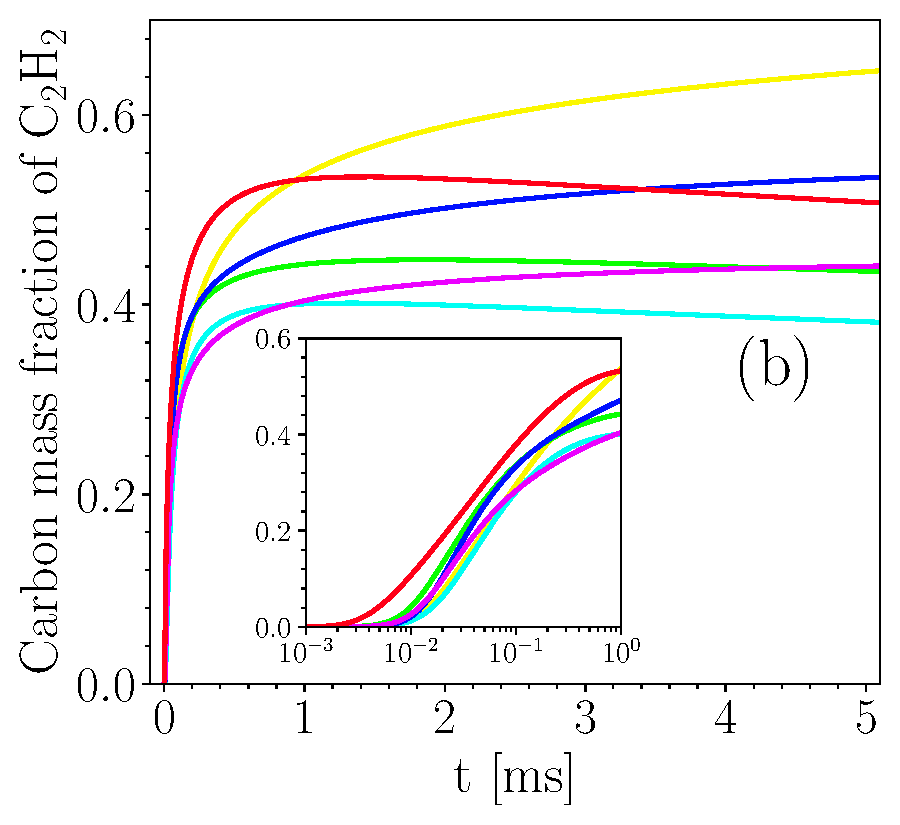
\includegraphics[width=1\textwidth]{Figures/Results/chemistry/C2H2.pdf}
	\end{subfigure}
	\caption{The mole fraction of $\mathrm{CH_4}$ (a), $\mathrm{C_2H_4}$ (b), and $\mathrm{C_2H_2}$ (c) during pyrolysis of 5\%~$\mathrm{CH_4}$-Ar predicted using different reaction mechanisms and compared with measurements~\hl{GB}. The insets provide a zoomed-in view of the early-time behavior and the shaded area represents the uncertainty in the reported experimental data.}
	\label{fig:CH4_C2H2_C2H4_chem} 
\end{figure}

As mentioned before, there is a large uncertainty in inception and PAH adsorption rates used PAH growth models. The default values were determined by applying the model to certain targets that vary for each model (some of the references can be found in Sections~\ref{sec:ebrimod} and \ref{sec:irrevdim}–\ref{sec:dimcoal} in which these models are explained). As a results, we do not focus on absolute accuracy of the models and instead use them to provide insight into the effect of chemistry and working parameters such as temperature and composition.
Here, Irreversible Dimerization model with 100\% efficiency of inception and PAH adsorption (i.e., all collisions result in inception and surface growth) is used to compare the maximum possible yield (represented by soot volume fraction) as an upper limit predicted by the selected mechanisms (except for FFCM2) during $5\%$ $\mathrm{CH_4}$ pyrolysis at $\mathrm{T_5}=$2203 K and $\mathrm{P_5}=$4.9 atm. 


As shown in Figure~\ref{fig:max_sootfv_chem}, the maximum possible $f_v$ predicted by ABF mechanism is lower than the measured $f_v$ considering the reported uncertainty. The same analysis was performed for other data points with a different $\mathrm{T_5}$ in~\hl{[G]}, and similar results were observed indicating that ABF mechanism cannot provide enough precursors under pyrolysis conditions in these simulations. In contrast, the maximum possible $f_v$ predicted by other mechanisms is significantly larger than the measurements, which presents the possibility of predicting $f_v$ close to the measurements using more realistic assumptions (i.e., lower dimerization efficiencies). Caltech and KAUST mechanisms are used in the simulations of this study for description of gas chemistry as they provide the highest carbon flux to soot precursors. ITV and CRECK mechanisms can also provide large enough precursors, but they are not used because of their large size that making parametric studies computationally expensive. Moreover, the selected mechanisms does not change the main findings about the difference between inception models in terms of temperature and composition sensitivity.

In the rest of presented results, the inception flux and PAH adsorption rate of PAH growth models are adjusted by calibrating $\eta_{inc}$ and $\eta_{ads}$ to match simulated soot with the available measurements. Note that, this approach does not resolve the mechanistic uncertainties of soot formation. It allows the model to calculate effective carbon fluxes from the gas phase into the particle phase that are consistent with measured soot characteristics.